\documentclass[letterpaper,12pt,twocolumn]{article}

\usepackage{amsmath,amssymb,mathpazo,xcolor,geometry,graphicx}
\geometry{top=0.75in,bottom=0.75in,right=0.75in,left=0.75in}
\graphicspath{../figures/}

\usepackage{biblatex}[backend=biber,citestyle=chicago-authordate]
\addbibresource{project2.bib}

\title{\Large Alternative Bandwidth Optimization Methods for Geographically Weighted Regression}
\author{Tyler D. Hoffman}
\date{3 December 2021}

\usepackage{hyperref}
\begin{document}
\maketitle

\section{Introduction}
\label{sec:introduction}
Geographically weighted regression (GWR; \cite{Fotheringham2003}) is a widely used statistical technique for analyzing spatial process variation and spatial relationships. The framework broadens a classical regression by allowing for spatially varying coefficients that illustrate different effects in different areas of the spatial domain. These coefficients are calibrated alongside a bandwidth parameter that controls the amount of spatial contextual information at a given location. During the fitting procedure, a local regression is fitted at every spatial observation using the information allotted by the bandwidth. Due to the influence it has on this process, the bandwidth parameter can be thought of as an indicator of the scale at which the process operates.

To find the bandwidth parameter, the fitting procedure makes use of a version of the Akaike information criterion (AIC; \cite{Akaike1973}) that incorporates a penalty term to disincentivize overly complex models. The GWR-corrected AIC, or AICc, takes the form \cite{Fotheringham2003} \begin{align*}
    \text{AICc} = -2\log f(y | \beta, \sigma^2, X) + \frac{2n(k+1)}{n-k-2}
\end{align*} where $f(y | \beta, \sigma^2, X)$ is the likelihood function for the model, $n$ is the number of observations (i.e., areal units), and $k$ is the effective number of parameters for the model. This paper regards the AICc as a function of the GWR bandwidth, which controls the amount of data used at a given observation to calibrate its local model. In GWR, the optimal bandwidth---the bandwidth that the model ultimately reports---is the one that minimizes the AICc.

Theoretically, this minimization problem is easy to frame. In practice, however, the computation can get messy. Since the AICc does not have an analytical derivative with respect to the bandwidth, one must use a derivative-free optimization method to find its minimizer. As a consequence, the performance of this optimizer is severely constrained: no derivative information means that an optimization method must learn the shape of the objective on its own or use heuristic or naive methods to find a minimum. These handicaps can be costly in terms of performance and make it difficult to quickly and accurately solve the minimization problem.

Additional constraints or information about an optimization problem always help refine the optimization strategy. By exploiting elements of the problem's structure, it is possible to customize faster and more powerful optimization methods. Such information is even more important when the objective lacks a derivative, as the optimizers must make up for not knowing the slope of the function.

While many improvements have been made to GWR since its inception (in particular, the generalization of the method into MGWR \cite{Oshan2019}), this paper focuses on the original procedure for simplicity. Indeed, this paper aims to deconstruct the optimization procedure for the GWR bandwidth and to examine the interplay between the structure of the problem and solution methods. By analyzing the problem's structure, it is possible to extract more insights about viable research directions for more efficient and reliable optimization techniques.

\section{Problem Structure}
\label{sec:problem}
Following ideas developed in \cite{Hoffman2021}, it is natural to consider the AICc as a combination of two terms acting independently: the log-likelihood, as a proxy for model fit, and the GWR correction, as a penalty for overfitting. Both of these vary as a function of bandwidth, but the way in which they vary differs between the two.

\begin{itemize}
    \item Decompose the AICc
    \item Outline the three components that really affect optimization here: minima, steepness, and noise
\end{itemize}

\subsection{Minima}
\begin{itemize}
    \item start with what we know (first three bullets on that slide) which is the foundation for how GWR works
    \item spend some time discussing multiple minimizers
    \item explain why this is dangerous for an optimizer / how an optimizer should account for it
\end{itemize}

\subsection{Steepness}
\begin{itemize}
    \item Emphasize that due to fixed (monotonic) nature of the correction, the steepness is nearly completely determined by the log-likelihood. Process variation is the name of the game
    \item Bandwidth CI issues---CIs can be wide even if the optimum is well-defined. How does Golden section search address this at present?
    \item explain why this is dangerous for an optimizer / how an optimizer should account for it   
\end{itemize}

\subsection{Noise}
\begin{itemize}
    \item explain the way that noise develops in these curves---due to the way areal units work
    \item explain why this is dangerous for an optimizer / how an optimizer should account for it
\end{itemize}

\section{Methods}
\label{sec:methods}
\subsection{Optimizers}
This work tests four optimizers for finding the optimal bandwidth. First, grid search (brute force optimization) is presented as a baseline for performance benchmarking. Next, a version of golden-section search \cite{Kiefer1953} similar to the implementation in the Python \texttt{mgwr} module was tested \cite{Oshan2019}. Golden-section search looks for the minimum of a unimodal function in a specified interval by repeatedly bisecting that interval according to the golden ratio ($\phi = (1 + \sqrt{5})/2$). By enforcing this proportion, the search algorithm offers a good rate of convergence to the minimum without sacrificing much in the way of accuracy. However, when applied to multimodal functions such as the AICc curve, golden-section search is known to get trapped in local minima. One proposal to avoid this is to use different initial points for golden-section search and to use the best result. More research is required to determine what guarantees this lends to the search method.

Another prototypical derivative-free optimizer, Brent's method, was also tested \cite{Brent1973}. Brent's method combines the bisection method and a quadractic version of the secant method (inverse quadractic interpolation instead of linear interpolation) by testing how much each method improved the solution at each iteration. By balancing the two, it has a worse worst-case complexity than the bisection method, but converges superlinearly if the objective is well-behaved.

Finally, particle swarm optimization (PSO) was considered as a heuristic approach to optimization \cite{Bonyadi2017}. PSO lets loose a swarm of particles (candidate solutions) in the domain which search for minima by moving with a certain amount of velocity. On each iteration, the particles use this built-in velocity, knowledge of their own best position, and knowledge of the swarm's best position to determine where to move. As a result, PSO can effectively explore local minima: as long as one particle reaches the absolute minimum, the swarm has succeeded. Additionally, due to the highly parallel behavior of the particles, PSO lends itself well to parallel computing implementations. These can improve the runtime of the algorithm, but do not improve the number of objective calls done by the algorithm. While these parallel methods are not explored in this paper, they could offer significant practical speedups in implementation.

\subsection{Sample Data}
As explained in Section \ref{sec:problem}, the AICc curves typically look like smooth checkmarks. The baseline curve (Figure \ref{fig:baseline}) was therefore chosen to be $b(x) = (x^2 - x + 600)/2x$ for $x > 0$ as it depicts well this smooth, unimodal shape. Subsequently, this objective was altered along the three axes of study: minima, steepness, and noise. All experiments were conducted with a low amount of added noise to simulate how real AICc curves behave.

To introduce multiple minima, a rule was prescribed that adds more checkmark-shaped curves along fixed displacements (Figure \ref{fig:multiple-mins}). The extra checkmarks take the form \begin{align*}
    g(x) = 0.0005((x-120)/10)^8 + x - 65
\end{align*} and for a given set of new minima locations $\{a_i\}_{i=1}^m$ were displaced to create a set of functions \begin{align*}
    h_i(x) = g(x - a_i) + a_i/2, i = 1, \dots, m.
\end{align*} Finally, for each $x$, the multiple minimum objective was defined as \begin{align*}
    b_m(x) = \min \{b(x), h_1(x), \dots, h_m(x)\} + \text{noise}.
\end{align*} 

For steepness, the baseline curve was parametrized with an additional steepness factor that altered the slope of the curve's tail (Figure \ref{fig:steep-curves}). These curves took the form \begin{align*}
    b_\sigma(x) = (\sigma x^2 - x + 600)/2x
\end{align*} where $\sigma > 0$ was the steepness parameter.

To add the noise, the generalized Hénon map was used \cite{Henon1976}. The noise needed to be non-random so it could be controlled across all optimizers, so a hyperchaotic dynamical system was utilized to ensure the noise could not be predicted but were replicable. The discrete-time dynamical system takes the form \begin{align*}
    x_i = a - x_{i-1}^2 - bx_{i-2}
\end{align*} where $a = 1.76$ and $b = 0.1$ are taken to be fixed parameters that are known to generate hyperchaos. To generate the noise, the system was run for 100 iterations using initial conditions $x_0 = 0$ and $x_1 = x$, where $x$ is the point for which the noise was requested (Figure \ref{fig:noisy-curves}). 

\begin{figure}
    \centering
    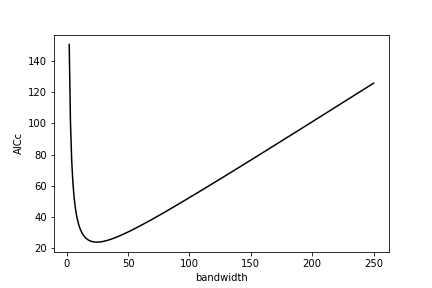
\includegraphics[width=0.5\textwidth]{../figures/baseline.png} 
    \caption{The base curve used for the numerical experiments.}
    \label{fig:baseline}
\end{figure}

\section{Results and Discussion}
\label{sec:results}
present results and explain what they mean. time/accuracy tradeoff (obv)

\section{Conclusion}
\label{sec:conclusion}
conclude, discuss limitations of this, and point to future work

\printbibliography
\pagebreak

\onecolumn
\section*{Large Figures}
\label{sec:figs}

\begin{figure}[h!]
    \centering
    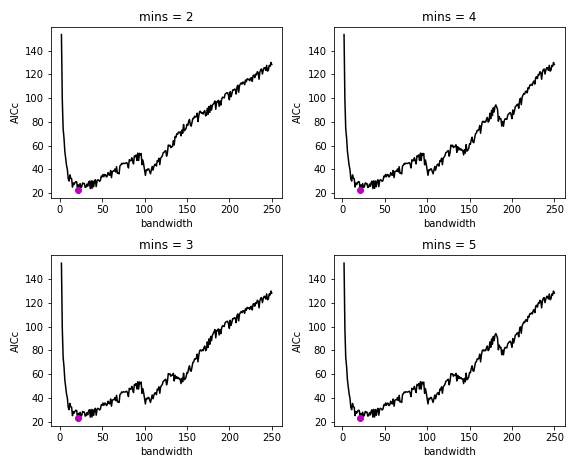
\includegraphics[width=\textwidth]{../figures/multiple-mins-curves.png}
    \caption{Examples of four numbers of minima used in the numerical experiments.}
    \label{fig:multiple-mins}
\end{figure}

\begin{figure}
    \centering
    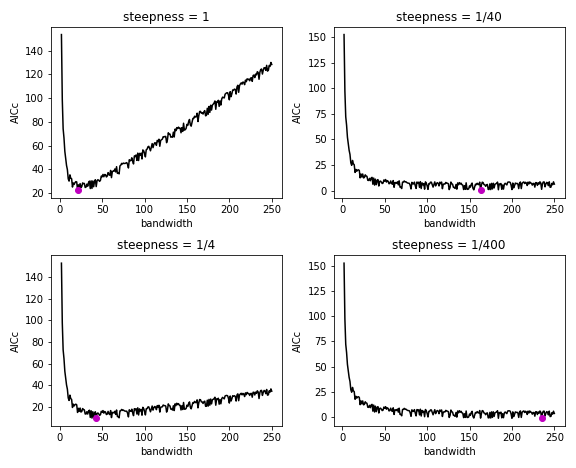
\includegraphics[width=\textwidth]{../figures/steep-curves.png}
    \caption{Examples of four steepness levels used in the numerical experiments.}
    \label{fig:steep-curves}
\end{figure}

\begin{figure}
    \centering
    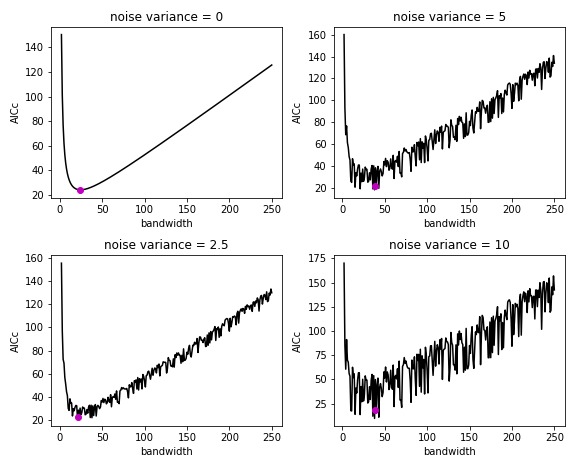
\includegraphics[width=\textwidth]{../figures/noisy-curves.png}
    \caption{Examples of four noise levels used in the numerical experiments.}
    \label{fig:noisy-curves}
\end{figure}

\end{document}